% !TeX program = xelatex
% Biên dịch trong thư mục report: xelatex bmp_report.tex (chạy hai lần).
% Dùng phông Unicode riêng thay cho STIX kiểu cũ do cas-sc nạp mặc định.
\PassOptionsToPackage{nomath,notext}{stix}
\documentclass[a4paper,fleqn]{cas-sc}
\usepackage{fontspec}
\IfFontExistsTF{Times New Roman}{\setmainfont{Times New Roman}}{\setmainfont{TeX Gyre Termes}}
\IfFontExistsTF{Arial}{\setsansfont{Arial}}{\setsansfont{TeX Gyre Heros}}
\IfFontExistsTF{Consolas}{\setmonofont{Consolas}[Scale=MatchLowercase]}{\setmonofont{TeX Gyre Cursor}[Scale=MatchLowercase]}
\usepackage{unicode-math}
\setmathfont{Latin Modern Math}
\usepackage[numbers,sort&compress]{natbib}
\usepackage{longtable}
\usepackage{placeins}
\usepackage{float}
\usepackage{enumitem}
\geometry{a4paper,left=22mm,right=22mm,top=22mm,bottom=22mm}
\renewcommand{\figurename}{Hình}
\renewcommand{\tablename}{Bảng}
\renewcommand{\refname}{Tài liệu tham khảo}
\renewcommand{\abstractname}{Tóm tắt}
\setlength{\parindent}{1.2em}
\setlength{\parskip}{2pt}
\setlength{\emergencystretch}{2em}
\setlist{nosep,leftmargin=1.8em}
\RenewDocumentCommand\printorcid{}{}
\ExplSyntaxOn
\cs_set:Npn \__first_footerline: {\small\sffamily Báo~cáo~bài~tập~lớn:~Bandwidth~Minimization}
\cs_set:Npn \__first_foot: {\parbox[t]{\textwidth}{\rule{\textwidth}{.2pt}\\
  \__first_footerline: \hfill Trang~\thepage~/~\lastpage}}
\cs_set_eq:NN \__cas_foot: \__first_foot:
\ExplSyntaxOff
\pagestyle{cas}
\hypersetup{pdftitle={Nghiên cứu giải bài toán Bandwidth Minimization bằng SAT và so sánh với CP, MIP, memeo},
  pdfauthor={Phạm Đức Hùng, Trần Nhật Hưng, hehe},unicode=true}
\graphicspath{{../results/visualization/png/}}
\newcommand{\code}[1]{\nolinkurl{#1}}
\newcommand{\figreport}[4]{%
  \begin{figure}[pos=!htbp]\centering
  \includegraphics[width=#2\linewidth]{#1}
  \caption{#3}\label{#4}
  \end{figure}}


\begin{document}
\shorttitle{Giải bài toán BMP bằng SAT và so sánh đa mô hình}
\shortauthors{Phạm Đức Hùng, Trần Nhật Hưng, Phạm Hồng Nam}
\title[mode=title]{Nghiên cứu giải bài toán Bandwidth Minimization bằng SAT: so sánh mã hóa Pairwise, Order và các mô hình CP, MIP}
\author[1]{Phạm Đức Hùng}
\author[1]{Trần Nhật Hưng}
\author[1]{Phạm Hồng Nam}
\affiliation[1]{organization={Khoa Công nghệ Thông tin, Trường Đại học Công nghệ, Đại học Quốc gia Hà Nội},
  city={Hà Nội},country={Việt Nam}}
\begin{abstract}
Bài toán Bandwidth Minimization (BMP) tìm một hoán vị các đỉnh của đồ thị sao cho khoảng cách lớn nhất giữa hai đầu mút của một cạnh là nhỏ nhất. Báo cáo nghiên cứu phương pháp giải chính xác dựa trên SAT, sử dụng hai mã hóa Pairwise và Order kết hợp với hai chiến lược SAT nhiều lần và Incremental SAT. Năm kỹ thuật mã hóa ràng buộc At-Most-One được cài đặt và khảo sát gồm Binomial, Binary, Commander, Product và Sequential. Thực nghiệm sử dụng 113 đồ thị Harwell--Boeing trong dự án, với giới hạn 120 giây và 8 GiB RAM cho mỗi lượt chạy. Kết quả cho thấy Product đạt bandwidth tốt nhất quan sát được, kể cả hòa, trên 83/113 đồ thị trong nhóm AMO; Sequential có số lượt chứng minh tối ưu cao nhất trong nhóm này, với 7 lượt. Với Pairwise + Product, Incremental tìm được bandwidth nhỏ hơn SAT nhiều lần trên 77/113 đồ thị. Mã hóa Order hiện tại gặp giới hạn bộ nhớ do phần ràng buộc hoán vị có số mệnh đề bậc ba theo số đỉnh. Khi so sánh năm phương pháp SAT, IBM CP Optimizer, IBM CPLEX MIP, OR-Tools CP-SAT và Gurobi, CP đạt hoặc hòa bandwidth tốt nhất trên cả 113 đồ thị, nhưng chỉ có 6 lượt được chính phương pháp này chứng minh tối ưu. Báo cáo phân biệt chất lượng nghiệm, độ bao phủ và khả năng chứng minh tối ưu; đồng thời phân tích ảnh hưởng của chi phí dựng mô hình, cận dưới và quy tắc xử lý các lượt không thành công.
\end{abstract}
\begin{keywords}
Bandwidth Minimization \sep SAT \sep Incremental SAT \sep Order encoding \sep At-Most-One \sep Constraint Programming \sep Mixed-Integer Programming
\end{keywords}
\maketitle

\section{Giới thiệu}
Các bài toán bố trí đồ thị xuất hiện khi cần gán vị trí cho các đối tượng có quan hệ với nhau. Trong BMP, vị trí là các số nguyên liên tiếp và chi phí của một cách bố trí được quyết định bởi cạnh có hai đầu mút xa nhau nhất. Dưới góc nhìn ma trận, việc đổi thứ tự các đỉnh tương đương với hoán vị đồng thời các hàng và cột của ma trận kề; mục tiêu là đưa các phần tử khác không lại gần đường chéo chính. Hình~\ref{fig:example} minh họa điều này trên một đường đi sáu đỉnh.

Torres-Jimenez và cộng sự~\cite{torres2015} nghiên cứu BMP bằng thuật toán luyện kim mô phỏng biểu diễn kép DRSA. Bài báo cung cấp định nghĩa bài toán, bối cảnh ứng dụng và bộ đối chuẩn Harwell--Boeing gồm 113 trường hợp. Định hướng của nghiên cứu hiện tại là xây dựng các mô hình giải chính xác, trong đó một nghiệm khả thi và một chứng minh tối ưu là hai kết quả cần được phân biệt. Khi bị giới hạn thời gian, một phương pháp giải chính xác vẫn có thể chỉ trả về nghiệm khả thi.

Báo cáo kế thừa cách trình bày và hướng nghiên cứu các mã hóa AMO từ báo cáo N-Queens giữa kỳ~\cite{hungNQueens}. Tuy nhiên, N-Queens chủ yếu yêu cầu tìm một cách đặt hậu hợp lệ, còn BMP có hàm mục tiêu cần giảm liên tục. Tìm được một hoán vị hợp lệ cho BMP tương đối dễ; cải thiện bandwidth và chứng minh không tồn tại hoán vị tốt hơn mới là nhiệm vụ khó. Vì vậy, không thể chuyển trực tiếp các kết luận về thời gian tìm nghiệm của N-Queens sang bài toán tối ưu BMP.

Nghiên cứu tập trung vào ba câu hỏi: (i) kỹ thuật AMO nào hỗ trợ tốt cho mô hình Pairwise trong ngân sách hiện có; (ii) hai mã hóa Pairwise, Order và hai chiến lược SAT nhiều lần, Incremental khác nhau như thế nào; (iii) mô hình SAT đã chọn có chất lượng nghiệm, khả năng chứng minh tối ưu và nhu cầu tài nguyên ra sao khi đặt cạnh CP và MIP. Các đóng góp thực hiện trong dự án gồm mã hóa CNF, giải mã và kiểm chứng nghiệm độc lập, bộ điều khiển benchmark có giới hạn tài nguyên, cùng các bảng và biểu đồ được tạo từ dữ liệu đo thực tế.

\figreport{bmp_matrix_example.png}{0.81}{Ma trận kề của cùng một đường đi sáu đỉnh trước và sau khi đổi thứ tự.}{fig:example}

\section{Bài toán và cơ sở nghiên cứu}
\subsection{Định nghĩa toán học}
Cho đồ thị vô hướng đơn $G=(V,E)$, với $|V|=n$, $|E|=m$. Một cách đánh số là song ánh $\pi:V\rightarrow\{1,\ldots,n\}$. Bandwidth của cách đánh số đó là
\begin{equation}
 B(\pi)=\max_{\{u,v\}\in E}|\pi(u)-\pi(v)|,\qquad
 B^*(G)=\min_{\pi\text{ là song ánh}}B(\pi).
\label{eq:bmp}
\end{equation}
Với đồ thị không có cạnh, quy ước $B(\pi)=0$. Mọi hoán vị đều khả thi và cho một cận trên; đặc biệt, $0\leq B^*(G)\leq n-1$. Trong mã nguồn, thứ tự đỉnh gốc $1,\ldots,n$ được dùng để tính cận trên khởi đầu $U_0$. Cận này có thể lớn hơn đáng kể so với giá trị tối ưu.

Vậy liệu tồn tại $\pi$ thỏa $B(\pi)\leq k$ hay không? Ký hiệu công thức CNF biểu diễn câu hỏi này là $F_k$. Khi $F_k$ thỏa được, ta có một cận trên; khi $F_{k-1}$ không thỏa được và đã có nghiệm bandwidth $k$, giá trị tối ưu là $k$.

\subsection{Các cận dưới được sử dụng}
Nhóm so sánh liên mô hình dùng cận dưới đồ thị $L_0$ chung, được lấy bằng giá trị lớn nhất của ba cận:
\begin{align}
 L_{\deg}&=\left\lceil\Delta(G)/2\right\rceil,\nonumber\\
 L_{\mathrm{ball}}&=\max_{v\in V,\,1\leq r\leq3}
       \left\lceil\frac{|N_{\leq r}(v)|-1}{2r}\right\rceil,\nonumber\\
 L_{\mathrm{clique}}&=|C_{\mathrm{greedy}}|-1,\qquad
 L_0=\max\{L_{\deg},L_{\mathrm{ball}},L_{\mathrm{clique}}\}.
\label{eq:bounds}
\end{align}
Ở đây $N_{\leq r}(v)$ gồm cả $v$ và các đỉnh cách $v$ không quá $r$ cạnh. Nếu bandwidth không quá $B$, các đỉnh này phải nằm trong một khoảng có nhiều nhất $2rB+1$ vị trí; từ đó suy ra cận lân cận. Một clique gồm $q$ đỉnh đòi hỏi hai vị trí cực trị cách nhau ít nhất $q-1$. Mã nguồn tìm clique bằng thuật toán tham lam, nên $C_{\mathrm{greedy}}$ là một clique tìm được, không được mặc nhiên xem là clique lớn nhất.

Trong quá trình giải, CP và MIP có thể nâng cận dưới bằng suy luận nội bộ. Cột \code{lower_bound} lưu cận đã ghi nhận, ít nhất bằng $L_0$ khi dữ liệu hợp lệ. Do đó, cận dưới cuối cùng của các phương pháp trên cùng đồ thị có thể khác nhau.

\section{Mã hóa SAT và chiến lược tối ưu}

\subsection{Mã hóa Pairwise với biến gán vị trí}

Để giải bài toán BMP bằng SAT, trước tiên cần biểu diễn việc sắp xếp các đỉnh thành các biến Boolean.

Với đồ thị có $n$ đỉnh, ta tạo biến $x_{v,p}$ với ý nghĩa:
\begin{equation*}
x_{v,p} =
\begin{cases}
1, & \text{nếu đỉnh } v \text{ được đặt ở vị trí } p,\\
0, & \text{ngược lại}.
\end{cases}
\end{equation*}

Ví dụ, nếu $x_{2,4}=1$, nghĩa là đỉnh số 2 được đặt ở vị trí thứ 4 trong hoán vị.

Để các biến này biểu diễn một hoán vị hợp lệ, cần thỏa mãn hai điều kiện: Mỗi đỉnh phải được gán vào đúng một vị trí và mỗi vị trí chỉ được chứa đúng một đỉnh. Hai điều kiện được biểu diễn bằng:
\begin{equation}
\bigwedge_{v\in V}
\operatorname{ExactlyOne}(x_{v,1},\ldots,x_{v,n})
\ \land\
\bigwedge_{p=1}^{n}
\operatorname{ExactlyOne}(x_{1,p},\ldots,x_{n,p}).
\label{eq:eo}
\end{equation}

Ràng buộc Exactly-One được tạo thành từ hai ràng buộc nhỏ hơn là At-Least-One (ALO) và At-Most-One (AMO). Trong đó, ALO yêu cầu ít nhất một biến nhận giá trị đúng, còn AMO yêu cầu không có hai biến nào đồng thời nhận giá trị đúng.

Ví dụ, với ba biến $x_1,x_2,x_3$, ALO yêu cầu ít nhất một biến đúng, còn AMO không cho phép hai biến cùng đúng. Kết hợp hai điều kiện, ta có đúng một biến nhận giá trị đúng.

Sau khi bảo đảm mỗi đỉnh có một vị trí duy nhất, ta cần giới hạn khoảng cách giữa các đỉnh kề nhau. Với mỗi cạnh $\{u,v\}$, hai đỉnh $u$ và $v$ phải được đặt tại các vị trí cách nhau không quá $k$. Nếu hai vị trí $p$ và $q$ có $|p-q|>k$, ta không cho phép $u$ và $v$ đồng thời được gán vào hai vị trí đó.

Ràng buộc SAT tương ứng là:
\begin{equation}
\neg x_{u,p}\lor\neg x_{v,q}.
\label{eq:pair-edge}
\end{equation}

Ví dụ, nếu $k=2$ thì hai đỉnh có cạnh nối không được đồng thời nằm tại vị trí 1 và 4, vì khoảng cách giữa chúng bằng 3.

Trong dự án này, Pairwise là tên của phương pháp biểu diễn vị trí đỉnh và cấm các cặp vị trí không hợp lệ trên mỗi cạnh. Trong khi đó, Binomial là một kỹ thuật cụ thể để mã hóa ràng buộc AMO. Vì vậy, cấu hình Pairwise + Product vẫn sử dụng các biến $x_{v,p}$ và ràng buộc cạnh như trên, nhưng dùng Product thay cho Binomial để mã hóa AMO.


Về kích thước công thức, Pairwise Encoding sử dụng $n^2$ biến Boolean ban đầu để biểu diễn việc gán $n$ đỉnh vào $n$ vị trí. Ngoài ra, tùy theo kỹ thuật AMO được lựa chọn, mô hình có thể cần thêm các biến phụ. Tổng số mệnh đề CNF bao gồm $2n$ mệnh đề ALO, $2n$ nhóm ràng buộc AMO và các mệnh đề giới hạn bandwidth trên từng cạnh. Gọi $C_{\mathrm{AMO}}(n)$ là số mệnh đề cần thiết để mã hóa một AMO có $n$ biến đầu vào, tổng số mệnh đề của Pairwise được tính bởi:
\begin{equation}
C_{\mathrm{Pairwise}}(n,m,k)
=2n+2nC_{\mathrm{AMO}}(n)+m(n-k-1)(n-k).
\label{eq:pairwise-size}
\end{equation}

Nếu sử dụng Binomial, mỗi AMO tạo ra $\binom{n}{2}$ mệnh đề và không cần biến phụ. Khi đó, tổng số mệnh đề là:
\begin{equation}
C_{\mathrm{Pairwise+Binomial}}(n,m,k)
=2n+2n\binom{n}{2}+m(n-k-1)(n-k).
\end{equation}

Trong khi đó, nếu sử dụng Product, phần ràng buộc AMO được thay thế bằng cấu trúc hàng--cột có biến phụ nhằm giảm số mệnh đề. Thành phần ràng buộc cạnh vẫn giữ nguyên, do đó kích thước CNF phụ thuộc cả vào phương pháp mã hóa AMO và ngưỡng bandwidth $k$. Khi $k$ giảm, số cặp vị trí không hợp lệ tăng lên, làm số mệnh đề ràng buộc cạnh tăng theo.

\subsection{Năm kỹ thuật mã hóa AMO}

Ràng buộc At-Most-One (AMO) yêu cầu trong một nhóm biến Boolean có nhiều nhất một biến nhận giá trị đúng. Với $q$ biến $z_1,z_2,\ldots,z_q$, điều kiện AMO được biểu diễn bởi:
\[
\sum_{i=1}^{q}z_i\leq 1.
\]

Ví dụ, với ba biến $z_1,z_2,z_3$, cách gán $(1,0,0)$ là hợp lệ, trong khi $(1,1,0)$ không hợp lệ vì có hai biến cùng đúng. Có nhiều phương pháp chuyển AMO thành công thức CNF, khác nhau chủ yếu ở số biến phụ, số mệnh đề và cách tổ chức các ràng buộc. Trong dự án, nhóm cài đặt năm phương pháp mã hóa trong thư mục \code{src/encodings/cardinality}. Thư viện PySAT~\cite{pysat} được sử dụng để gọi SAT Solver giải công thức CNF.

\subsubsection{Binomial Encoding}

Binomial là phương pháp mã hóa trực tiếp và dễ hiểu nhất. Ý tưởng là không cho phép bất kỳ hai biến đầu vào nào đồng thời nhận giá trị đúng. Với mỗi cặp biến $z_i,z_j$, phương pháp thêm một mệnh đề:
\[
\neg z_i\lor\neg z_j,\qquad i<j.
\]

Ví dụ, với ba biến $z_1,z_2,z_3$, công thức CNF được tạo thành:
\[
(\neg z_1\lor\neg z_2)\land(\neg z_1\lor\neg z_3)\land(\neg z_2\lor\neg z_3).
\]

Như vậy, nếu một biến nhận giá trị đúng thì tất cả các biến còn lại bắt buộc phải sai. Ưu điểm của Binomial là không cần sử dụng biến phụ, công thức đơn giản và dễ kiểm tra. Tuy nhiên, số mệnh đề cần tạo là:
\[
\binom{q}{2}=\frac{q(q-1)}{2}.
\]

Do đó, khi số biến đầu vào tăng, số mệnh đề tăng nhanh theo bậc hai. Trong mô hình hoán vị của Pairwise Encoding, có tổng cộng $2n$ ràng buộc AMO, mỗi ràng buộc chứa $n$ biến. Vì vậy, nếu toàn bộ AMO đều sử dụng Binomial, tổng số mệnh đề AMO tăng theo bậc ba của $n$.

\subsubsection{Binary Encoding}

Binary sử dụng các biến phụ để biểu diễn chỉ số của biến đầu vào được phép nhận giá trị đúng. Thay vì cấm trực tiếp từng cặp biến như Binomial, phương pháp gán cho mỗi biến đầu vào một mã nhị phân riêng biệt. Với $q$ biến đầu vào, số bit phụ cần sử dụng là:
\[
b=\lceil\log_2 q\rceil.
\]

Ví dụ, với bốn biến đầu vào, chỉ cần hai bit phụ để biểu diễn bốn mã nhị phân khác nhau:
\[
z_1\rightarrow 00,\quad z_2\rightarrow 01,\quad z_3\rightarrow 10,\quad z_4\rightarrow 11.
\]

Khi một biến $z_i$ đúng, các bit phụ bắt buộc phải nhận đúng mã nhị phân tương ứng. Nếu hai biến đầu vào cùng đúng, chúng sẽ yêu cầu các bit phụ nhận hai mã khác nhau, dẫn đến mâu thuẫn. Do đó, không thể có hai biến đầu vào cùng nhận giá trị đúng. Ưu điểm của Binary là giảm số mệnh đề so với Binomial khi $q$ lớn. Mã hóa sử dụng $\lceil\log_2 q\rceil$ biến phụ và $q\lceil\log_2 q\rceil$ mệnh đề.

\subsubsection{Commander Encoding}

Commander chia tập biến đầu vào thành nhiều nhóm nhỏ để dễ quản lý. Trong mỗi nhóm, một biến phụ gọi là commande được sử dụng để đại diện cho nhóm đó. Thay vì tạo mệnh đề cấm trực tiếp giữa mọi cặp biến của toàn bộ tập đầu vào, phương pháp tổ chức các ràng buộc AMO theo nhiều cấp.

Đầu tiên, các biến đầu vào được chia thành những nhóm có tối đa ba biến. Trong mỗi nhóm, phương pháp áp dụng AMO để bảo đảm không có hai biến cùng đúng, đồng thời liên kết các biến đầu vào với commander tương ứng. Sau đó, AMO tiếp tục được áp dụng giữa các commander, có thể thực hiện đệ quy nếu số lượng commander còn lớn.

Nếu một biến đầu vào đúng, commander của nhóm chứa biến đó cũng phải đúng. Ràng buộc AMO giữa các commander sẽ ngăn hai nhóm khác nhau cùng chứa biến đầu vào đúng. Bản cài đặt trong dự án còn bổ sung chiều suy ra ngược lại, theo đó commander đúng thì phải có ít nhất một biến thuộc nhóm tương ứng đúng.

Ưu điểm của Commander là chia một ràng buộc lớn thành nhiều ràng buộc nhỏ, giúp tránh việc tạo mệnh đề cho mọi cặp biến trên toàn bộ tập đầu vào. Với kích thước nhóm cố định, số biến phụ và số mệnh đề đều tăng tuyến tính theo số biến đầu vào~\cite{commander}.

\subsubsection{Product Encoding}

Product cũng sử dụng các biến phụ để giảm số mệnh đề, nhưng khác Commander ở cách tổ chức các biến đầu vào. Cụ thể, phương pháp sắp xếp các biến thành một bảng gồm nhiều hàng và cột, sau đó tạo các biến phụ đại diện cho từng hàng và từng cột.

Ví dụ, với chín biến đầu vào, ta có thể sắp xếp chúng thành bảng $3\times3$:
\[
\begin{matrix}
z_1 & z_2 & z_3\\
z_4 & z_5 & z_6\\
z_7 & z_8 & z_9
\end{matrix}
\]

Mỗi hàng và mỗi cột được gắn với một biến phụ. Nếu một biến $z_i$ đúng thì biến phụ của hàng và cột chứa nó cũng phải đúng. Sau đó, phương pháp áp dụng AMO cho nhóm biến phụ hàng và nhóm biến phụ cột.

Ví dụ, nếu $z_1$ và $z_5$ cùng đúng thì chúng thuộc hai hàng và hai cột khác nhau. Khi đó, hai biến phụ hàng và hai biến phụ cột tương ứng sẽ cùng đúng, vi phạm các ràng buộc AMO. Tương tự, nếu hai biến nằm trên cùng một hàng nhưng khác cột thì AMO giữa các biến phụ cột sẽ ngăn chúng cùng đúng. Nhờ vậy, toàn bộ bảng chỉ có thể chứa nhiều nhất một biến đầu vào đúng.

Trong mã nguồn, nhóm lựa chọn số hàng và số cột gần bằng nhau theo công thức:
\[
h=\lfloor\sqrt q\rfloor,\qquad w=\left\lceil\frac{q}{h}\right\rceil.
\]

Cách phân chia này tiếp tục được áp dụng đệ quy cho các nhóm biến phụ. Với nhóm có nhiều nhất bốn biến, chương trình chuyển sang sử dụng Binomial. Ưu điểm của Product là sử dụng thêm biến phụ để giảm số mệnh đề so với Binomial. Với cách phân chia gần vuông và thực hiện đệ quy, số mệnh đề tăng tuyến tính theo $q$, trong khi số biến phụ tăng theo $O(\sqrt q)$~\cite{product}.

\subsubsection{Sequential Encoding}

Sequential xử lý các biến đầu vào theo thứ tự từ trái sang phải. Ý tưởng của phương pháp là sử dụng các biến phụ để ghi nhận liệu đã xuất hiện một biến đúng trong phần đầu của dãy hay chưa.

Ví dụ, xét bốn biến:
\[
z_1,z_2,z_3,z_4.
\]

Nếu $z_2=1$, mã hóa sẽ ghi nhận rằng đã xuất hiện một biến đúng trong phần đầu của dãy. Khi đó, các ràng buộc sẽ ngăn những biến phía sau như $z_3$ và $z_4$ tiếp tục nhận giá trị đúng.

Để thực hiện điều này, Sequential sử dụng các biến phụ $s_i$ nhằm ghi nhận trạng thái của các tiền tố. Các mệnh đề liên kết giữa những vị trí liên tiếp giúp duy trì thông tin về biến đã đúng. Cụ thể, mã hóa bắt đầu với mệnh đề $\neg z_1\lor s_1$. Với mỗi $2\leq i\leq q-1$, phương pháp bổ sung ba mệnh đề $\neg z_i\lor s_i$, $\neg s_{i-1}\lor s_i$ và $\neg z_i\lor\neg s_{i-1}$. Cuối cùng, mệnh đề $\neg z_q\lor\neg s_{q-1}$ bảo đảm biến cuối cùng không thể đúng nếu trước đó đã có một biến đúng.

Với $q\geq2$, Sequential sử dụng:
\[
q-1\text{ biến phụ},\qquad 3q-4\text{ mệnh đề}.
\]

Ưu điểm của Sequential là số mệnh đề tăng tuyến tính thay vì tăng theo bậc hai như Binomial. Đổi lại, phương pháp cần thêm các biến phụ để duy trì thông tin trong quá trình xử lý tuần tự~\cite{sinz}.

\subsubsection{So sánh kích thước các mã hóa}

Bảng~\ref{tab:amo-theory} tổng hợp số biến phụ và số mệnh đề CNF cần thiết để mã hóa một ràng buộc AMO có $q$ biến đầu vào, chưa tính mệnh đề ALO.

\begin{table}[pos=H]
\centering
\caption{So sánh kích thước của năm phương pháp mã hóa AMO.}
\label{tab:amo-theory}
\small
\begin{tabular}{lcc}
\toprule
\textbf{Mã hóa} & \textbf{Số biến phụ} & \textbf{Số mệnh đề} \\
\midrule
Binomial & $0$ & $\binom{q}{2}$ \\
Binary & $\lceil\log_2q\rceil$ & $q\lceil\log_2q\rceil$ \\
Commander (nhóm 3) & $O(q)$ & $O(q)$ \\
Product đệ quy & $O(\sqrt q)$ & $O(q)$ \\
Sequential ($q\geq2$) & $q-1$ & $3q-4$ \\
\bottomrule
\end{tabular}
\end{table}

Từ bảng trên, có thể thấy mỗi phương pháp mã hóa AMO đều có sự đánh đổi giữa số biến phụ và số mệnh đề cần tạo. Chẳng hạn, Binomial không sử dụng biến phụ nhưng có thể tạo ra rất nhiều mệnh đề. Trong khi đó, Binary, Commander, Product và Sequential sử dụng biến phụ để giảm số lượng mệnh đề, đồng thời làm thay đổi cấu trúc công thức CNF.

Tuy nhiên, công thức CNF nhỏ hơn không đồng nghĩa với việc SAT Solver luôn chạy nhanh hơn. Hiệu quả giải còn phụ thuộc vào cấu trúc mệnh đề, khả năng suy luận của solver, số biến phụ và độ khó của từng đồ thị. Vì vậy, nhóm tiến hành thực nghiệm cả năm phương pháp mã hóa AMO trên cùng tập đồ thị, cùng chiến lược tìm kiếm và giới hạn thời gian để lựa chọn phương pháp phù hợp cho các thí nghiệm SAT tiếp theo.



\subsection{Mã hóa Order bằng biến ngưỡng}

Khác với Pairwise Encoding, trong đó mỗi biến Boolean biểu diễn việc một đỉnh được gán vào một vị trí cụ thể, Order Encoding sử dụng các biến ngưỡng để biểu diễn vị trí của đỉnh. Cụ thể, biến $t_{v,p}$ nhận giá trị đúng khi đỉnh $v$ được đặt tại vị trí không lớn hơn $p$:
\[
t_{v,p}=1 \Longleftrightarrow \pi(v)\leq p.
\]

Ví dụ, xét đồ thị có 5 đỉnh. Nếu đỉnh $v$ được đặt tại vị trí thứ 3 thì các biến ngưỡng tương ứng nhận giá trị:
\[
(t_{v,1},t_{v,2},t_{v,3},t_{v,4},t_{v,5})=(0,0,1,1,1).
\]

Điều này có nghĩa là đỉnh $v$ không nằm trong hai vị trí đầu tiên, nhưng nằm trong phạm vi ba, bốn hoặc năm vị trí đầu. Như vậy, vị trí thực tế của một đỉnh được xác định tại thời điểm dãy biến chuyển từ False sang True.

Để biểu diễn đúng quy tắc trên, các biến của mỗi đỉnh phải có dạng một dãy False liên tiếp, sau đó là các giá trị True. Đồng thời, biến ở ngưỡng cuối cùng luôn phải đúng vì mọi đỉnh đều được đặt trong $n$ vị trí. Hai điều kiện này được biểu diễn bằng:
\begin{equation}
t_{v,n},\qquad \neg t_{v,p}\lor t_{v,p+1},\quad 1\leq p<n.
\label{eq:order-mono}
\end{equation}

Ràng buộc trên bảo đảm rằng nếu $t_{v,p}$ đã đúng thì $t_{v,p+1}$ cũng phải đúng. Nói cách khác, sau khi dãy chuyển sang True, nó không thể quay lại False. Nhờ đó, mỗi đỉnh có đúng một thời điểm chuyển từ False sang True, tương ứng với vị trí được gán trong hoán vị.


Các ràng buộc trên mới chỉ bảo đảm rằng mỗi đỉnh được gán vào một vị trí, nhưng chưa ngăn được trường hợp nhiều đỉnh cùng chiếm một vị trí. Vì vậy, Order Encoding cần bổ sung ràng buộc để mỗi vị trí chỉ có một đỉnh.

Theo cách biểu diễn bằng biến ngưỡng, một đỉnh $v$ nằm đúng tại vị trí $p$ khi $t_{v,p}$ nhận giá trị True và $t_{v,p-1}$ nhận giá trị False. Nói cách khác, vị trí của đỉnh được xác định tại điểm mà dãy biến ngưỡng chuyển từ False sang True. Ta quy ước $t_{v,0}=\mathrm{False}$ để áp dụng cách xác định này cho cả vị trí đầu tiên.

Ví dụ, nếu hai đỉnh $u$ và $v$ đều nằm ở vị trí 3 thì cả hai đều có $t_{u,2}=t_{v,2}=0$ và $t_{u,3}=t_{v,3}=1$. Điều này không hợp lệ vì hai đỉnh không được cùng chiếm một vị trí. Để loại bỏ trường hợp đó, với mỗi cặp đỉnh khác nhau $u,v$ và mỗi vị trí $p$, mô hình thêm mệnh đề:
\begin{equation}
\neg t_{u,p}\lor t_{u,p-1}\lor\neg t_{v,p}\lor t_{v,p-1}.
\label{eq:order-injective}
\end{equation}

Mệnh đề trên chỉ nhận giá trị False khi cả hai đỉnh cùng chuyển từ False sang True tại vị trí $p$. Khi đó, SAT Solver sẽ loại bỏ cách gán này. Nếu hai đỉnh nằm ở các vị trí khác nhau, mệnh đề vẫn được thỏa mãn. Riêng tại vị trí đầu tiên ($p=1$), do $t_{u,0}=t_{v,0}=\mathrm{False}$, công thức được rút gọn thành $\neg t_{u,1}\lor\neg t_{v,1}$.

Như vậy, kết hợp với điều kiện mỗi đỉnh có đúng một vị trí, ràng buộc này bảo đảm không có hai đỉnh nào chiếm cùng một vị trí. Do đồ thị có $n$ đỉnh và $n$ vị trí, kết quả thu được là một hoán vị hợp lệ.

Sau khi bảo đảm tính hợp lệ của hoán vị, mô hình cần bổ sung ràng buộc bandwidth. Với mỗi cạnh $\{u,v\}$, khoảng cách giữa vị trí của hai đỉnh phải không vượt quá ngưỡng $k$, tức là $|\pi(u)-\pi(v)|\leq k$. Trong Order Encoding, điều kiện này được biểu diễn bằng:
\begin{equation}
(\neg t_{u,p}\lor t_{v,p+k})\land
(\neg t_{v,p}\lor t_{u,p+k}),
\quad 1\leq p\leq n-k.
\label{eq:order-edge}
\end{equation}

Ý nghĩa của ràng buộc là nếu đỉnh $u$ nằm trong $p$ vị trí đầu tiên thì đỉnh $v$ phải nằm trong $p+k$ vị trí đầu tiên, và ngược lại. Ví dụ, nếu $k=2$ và đỉnh $u$ được đặt tại vị trí 3, thì đỉnh $v$ không được nằm sau vị trí 5. Áp dụng điều kiện theo cả hai chiều cũng ngăn $v$ nằm quá xa về phía trước $u$. Nhờ vậy, hai đỉnh có cạnh nối luôn cách nhau không quá $k$ vị trí. Những trường hợp có ngưỡng $p+k$ vượt quá $n$ không cần thêm mệnh đề vì mọi đỉnh đều nằm trong phạm vi $n$ vị trí.

Về kích thước công thức, Order Encoding trong dự án sử dụng $n^2$ biến Boolean và không cần các biến phụ AMO như một số cấu hình Pairwise. Tổng số mệnh đề được tạo ra với $0\leq k\leq n-1$ là:
\begin{equation}
C_{\mathrm{Order}}(n,m,k)
=n^2+n\binom{n}{2}+2m(n-k).
\label{eq:order-size}
\end{equation}

Trong công thức trên, $n^2$ mệnh đề dùng để bảo đảm dãy biến ngưỡng của mỗi đỉnh có dạng hợp lệ; $n\binom{n}{2}$ mệnh đề ngăn các cặp đỉnh cùng chiếm một vị trí; và $2m(n-k)$ mệnh đề dùng để giới hạn khoảng cách giữa các đỉnh có cạnh nối. Hai thành phần đầu không phụ thuộc vào $k$, trong khi thành phần cuối tăng khi ngưỡng bandwidth giảm.

Đáng chú ý, số mệnh đề ngăn các đỉnh trùng vị trí tăng theo bậc ba của $n$, tức là $\Theta(n^3)$. Điều này khiến công thức CNF có thể trở nên rất lớn khi số đỉnh tăng, dù mô hình chỉ sử dụng $n^2$ biến Boolean. Đây là đặc điểm của cách cài đặt Order Encoding hiện tại trong dự án, không có nghĩa mọi phương pháp mã hóa Order đều có cùng kích thước hoặc hiệu quả giải.



\subsection{SAT nhiều lần và Incremental SAT}

Để tìm bandwidth nhỏ nhất bằng SAT, nhóm sử dụng phương pháp kiểm tra lần lượt các ngưỡng $k$. Ban đầu, thuật toán tìm một hoán vị hợp lệ có bandwidth $U_0$, sau đó giảm $k$ từng đơn vị để kiểm tra xem có tồn tại hoán vị với bandwidth nhỏ hơn hay không. Nếu SAT Solver trả về SAT, nghĩa là tồn tại một hoán vị thỏa mãn ngưỡng đang xét và thuật toán tiếp tục giảm $k$. Ngược lại, nếu trả về UNSAT, nghĩa là không tồn tại hoán vị nào có bandwidth không vượt quá ngưỡng đó. Khi ngưỡng ngay trước đó có nghiệm, kết quả UNSAT cho phép khẳng định nghiệm tốt nhất đã tìm được là tối ưu.

Quá trình tìm kiếm cũng có thể dừng sớm khi nghiệm hiện tại đạt đến một cận dưới đã được chứng minh. Trong các thí nghiệm khảo sát kỹ thuật mã hóa AMO và so sánh các cấu hình SAT, thuật toán sử dụng cận dừng bằng 0. Khi so sánh SAT với các phương pháp tối ưu khác, nhóm sử dụng cận dưới đồ thị $L_0$ được xác định tại Công thức~\eqref{eq:bounds}. Bộ giải SAT được sử dụng là Glucose3 thông qua giao diện \code{Solver(name="g3")} của thư viện PySAT.

Hai chiến lược được khảo sát là SAT nhiều lần (Repeated SAT) và SAT tăng dần (Incremental SAT). Cả hai đều kiểm tra các ngưỡng bandwidth theo cùng một thứ tự, nhưng khác nhau ở cách quản lý công thức CNF và trạng thái của bộ giải.

\subsubsection{Repeated SAT}

Trong Repeated SAT, mỗi khi giảm ngưỡng $k$, chương trình xây dựng lại toàn bộ công thức CNF tương ứng và khởi tạo một SAT Solver mới. Solver kiểm tra công thức, trả về kết quả SAT hoặc UNSAT, sau đó được đóng trước khi chuyển sang ngưỡng tiếp theo.

Ưu điểm của cách tiếp cận này là đơn giản, dễ cài đặt và mỗi lần giải độc lập với các lần trước. Tuy nhiên, do phải tạo lại công thức và khởi tạo solver ở mọi ngưỡng, chương trình có thể tốn nhiều thời gian cho các thao tác lặp lại. Ngoài ra, những mệnh đề mà solver học được trong quá trình giải trước đó không được giữ lại để sử dụng ở ngưỡng tiếp theo.


\subsubsection{Incremental SAT}

Khác với Repeated SAT, Incremental SAT chỉ khởi tạo một SAT Solver duy nhất và tái sử dụng trong suốt quá trình tìm kiếm bandwidth tối ưu. Ban đầu, chương trình xây dựng công thức CNF hoàn chỉnh tại ngưỡng bandwidth $U_0$, bao gồm các ràng buộc hoán vị và ràng buộc khoảng cách giữa các đỉnh kề nhau. Công thức này được nạp vào solver để kiểm tra tính thỏa mãn. Khi giảm ngưỡng $k$, chương trình không xây dựng lại toàn bộ CNF mà chỉ sinh và bổ sung các mệnh đề ràng buộc cạnh cần thiết cho ngưỡng mới. Nhờ đó, các ràng buộc hoán vị, biến phụ AMO và những mệnh đề đã nạp trước đó được tái sử dụng, đồng thời solver có thể giữ lại thông tin học được từ các lần giải trước.

Đối với Pairwise Encoding, khi giảm ngưỡng từ $k+1$ xuống $k$, các cặp vị trí có khoảng cách lớn hơn $k+1$ đã bị cấm ở những lần giải trước. Vì vậy, chương trình chỉ cần bổ sung các mệnh đề cấm những cặp vị trí có khoảng cách đúng bằng $k+1$. Cách thực hiện này giúp tránh việc tạo lại các mệnh đề đã tồn tại và giảm chi phí xây dựng công thức CNF trong quá trình tìm kiếm.

Đối với Order Encoding, các mệnh đề ràng buộc cạnh phụ thuộc trực tiếp vào ngưỡng $k$, nên khi giảm ngưỡng, chương trình sinh các mệnh đề cạnh tương ứng với ngưỡng mới và bổ sung vào solver. Mặc dù những mệnh đề này có thể khác các mệnh đề ở ngưỡng trước về mặt cú pháp, chúng vẫn tương thích với các ràng buộc đã có vì ngưỡng bandwidth nhỏ hơn đặt ra điều kiện chặt hơn. Do đó, các mệnh đề cũ có thể được giữ lại mà không làm thay đổi tập nghiệm hợp lệ tại ngưỡng mới.

Nhờ chỉ xây dựng các ràng buộc hoán vị một lần và trực tiếp sinh các mệnh đề cạnh cần bổ sung, phiên bản Incremental SAT cải tiến giảm được chi phí tạo CNF và không cần sử dụng cấu trúc dữ liệu \code{set} để so sánh toàn bộ các mệnh đề qua từng ngưỡng. Tuy nhiên, số mệnh đề được lưu trong solver vẫn tăng dần khi ngưỡng bandwidth giảm, đặc biệt đối với Order Encoding. Bên cạnh đó, việc giảm thời gian xây dựng CNF không bảo đảm thời gian giải SAT hoặc chất lượng nghiệm luôn được cải thiện, do hiệu quả tìm kiếm còn phụ thuộc vào cấu trúc và thứ tự nạp mệnh đề cũng như cơ chế suy luận của solver.


\subsubsection{So sánh hai chiến lược}

Nhìn chung, Repeated SAT ưu tiên sự đơn giản và tính độc lập giữa các lần giải, trong khi Incremental SAT hướng đến việc tận dụng thông tin từ những lần giải trước để giảm công việc lặp lại. Tuy nhiên, Incremental SAT không nhất thiết luôn nhanh hơn Repeated SAT vì còn phụ thuộc vào chi phí xây dựng công thức, quản lý mệnh đề và khả năng tái sử dụng thông tin của solver. Do đó, nhóm tiến hành so sánh thực nghiệm hai chiến lược trên cùng tập dữ liệu và giới hạn thời gian để đánh giá hiệu quả thực tế.



\section{Các mô hình CP và MIP đối chứng}

Bên cạnh SAT, nhóm sử dụng thêm các phương pháp CP và MIP để giải bài toán Bandwidth Minimization Problem (BMP). Điểm khác biệt là các phương pháp này có thể trực tiếp tìm giá trị bandwidth nhỏ nhất, thay vì phải kiểm tra lần lượt từng ngưỡng $k$ như SAT. Các bộ giải được sử dụng gồm IBM CP Optimizer, Google OR-Tools CP-SAT, IBM CPLEX MIP và Gurobi.

\subsection{CP và CP-SAT}

Trong mô hình CP, mỗi đỉnh $v$ được gán một biến nguyên $p_v$ biểu diễn vị trí của đỉnh đó trong hoán vị, với $1\leq p_v\leq n$. Ví dụ, nếu $p_3=5$ thì đỉnh số 3 được đặt tại vị trí thứ 5.

Để bảo đảm các đỉnh không bị trùng vị trí, mô hình sử dụng ràng buộc \code{AllDifferent}, yêu cầu tất cả các biến vị trí phải có giá trị khác nhau. Vì đồ thị có $n$ đỉnh và $n$ vị trí, điều kiện này bảo đảm mỗi vị trí chứa đúng một đỉnh.

Tiếp theo, với mỗi cạnh $\{u,v\}$, khoảng cách giữa hai đỉnh được tính bằng $|p_u-p_v|$ và phải không vượt quá biến bandwidth $B$. Mục tiêu là tìm giá trị $B$ nhỏ nhất. Mô hình CP được biểu diễn như sau:
\begin{equation}
\begin{aligned}
\min\quad &B\\
\text{với}\quad
&\operatorname{AllDifferent}(p_1,\ldots,p_n),\\
&|p_u-p_v|\leq B,\quad \forall\{u,v\}\in E.
\end{aligned}
\label{eq:cp}
\end{equation}

Ví dụ, nếu hai đỉnh có cạnh nối được đặt tại vị trí 2 và 6 thì khoảng cách giữa chúng bằng 4. Khi đó, biến $B$ phải có giá trị ít nhất bằng 4 để thỏa mãn ràng buộc của cạnh này.

Mô hình OR-Tools CP-SAT sử dụng cùng cách biểu diễn vị trí và ràng buộc \code{AllDifferent}. Tuy nhiên, với mỗi cạnh $\{u,v\}$, chương trình tạo thêm biến $d_{uv}$ để lưu khoảng cách giữa hai đỉnh. Hàm \code{AddAbsEquality} được sử dụng để thiết lập $d_{uv}=|p_u-p_v|$, sau đó bổ sung điều kiện $d_{uv}\leq B$.

Như vậy, CP và CP-SAT đều tìm cách sắp xếp các đỉnh sao cho khoảng cách lớn nhất trên các cạnh là nhỏ nhất. Hai phương pháp khác nhau chủ yếu ở bộ giải và cơ chế tìm kiếm nghiệm bên trong~\cite{ortools,ibmcp}.

\subsection{MIP với CPLEX và Gurobi}

Hai bộ giải CPLEX MIP và Gurobi sử dụng cùng một mô hình quy hoạch nguyên hỗn hợp. Tương tự Pairwise SAT Encoding, mô hình tạo biến nhị phân $x_{v,p}$, trong đó $x_{v,p}=1$ nếu đỉnh $v$ được đặt tại vị trí $p$, và bằng 0 trong trường hợp ngược lại.

Vị trí của đỉnh $v$ được tính theo công thức:
\[
P_v=\sum_{p=1}^{n}p\,x_{v,p}.
\]

Ví dụ, nếu đỉnh $v$ nằm tại vị trí 3 thì $x_{v,3}=1$, các biến còn lại bằng 0 và ta có $P_v=3$.

Để tạo thành một hoán vị hợp lệ, mô hình yêu cầu mỗi đỉnh được gán vào đúng một vị trí và mỗi vị trí chứa đúng một đỉnh. Với mỗi cạnh $\{u,v\}$, khoảng cách giữa hai đỉnh phải không vượt quá bandwidth $B$. Mô hình được biểu diễn như sau:
\begin{align}
\min\quad &B,\nonumber\\
\sum_{p=1}^{n}x_{v,p}&=1 &&\forall v\in V,\nonumber\\
\sum_{v\in V}x_{v,p}&=1 &&\forall p=1,\ldots,n,\nonumber\\
P_u-P_v&\leq B,\quad P_v-P_u\leq B &&\forall\{u,v\}\in E.
\label{eq:mip}
\end{align}

Hai bất đẳng thức cuối được sử dụng thay cho điều kiện $|P_u-P_v|\leq B$, giúp biểu diễn giới hạn bandwidth bằng các ràng buộc tuyến tính. Mô hình sử dụng $n^2$ biến nhị phân, một biến nguyên $B$ và $2n+2m$ ràng buộc chính. Mặc dù mô hình MIP có số ràng buộc tương đối gọn, số lượng biến nhị phân tăng nhanh khi đồ thị lớn. Vì vậy, việc tìm nghiệm tốt và chứng minh nghiệm tối ưu vẫn có thể mất nhiều thời gian. Trong thực nghiệm, Gurobi được cấu hình với tham số \code{MIPFocus=3} và CPLEX MIP sử dụng \code{emphasis.mip=3}. Cả hai thiết lập đều hướng bộ giải tập trung hơn vào việc cải thiện cận dưới, hỗ trợ quá trình chứng minh nghiệm tối ưu.


\section{Thiết kế thực nghiệm}

\subsection{Dữ liệu và môi trường}

Các thí nghiệm được thực hiện trên bộ dữ liệu đồ thị Harwell--Boeing, sử dụng các tệp \code{.mtx.rnd} trong hai thư mục \code{data/hb_33} và \code{data/hb_80}. Bộ dữ liệu gồm tổng cộng 113 đồ thị, trong đó tập \code{hb_33} có 33 đồ thị và tập \code{hb_80} có 80 đồ thị. Các con số 33 và 80 biểu thị số lượng đồ thị trong từng tập, không phải số đỉnh của đồ thị.

Trước khi đưa vào các bộ giải, dữ liệu được chuẩn hóa thành đồ thị vô hướng đơn. Chương trình loại bỏ các cạnh nối một đỉnh với chính nó (self-loop), gộp các cạnh trùng lặp và giữ nguyên những đỉnh cô lập cũng như các thành phần liên thông. Bước chuẩn hóa giúp tất cả các phương pháp giải sử dụng cùng một biểu diễn đồ thị. Quy mô của hai tập dữ liệu được trình bày trong Bảng~\ref{tab:dataset}.

\begin{table}[pos=H]
\centering
\caption{Thống kê quy mô các đồ thị sau khi chuẩn hóa.}
\label{tab:dataset}
\small
\begin{tabular}{lrrrr}
\toprule
\textbf{Tập dữ liệu} & \textbf{Số đồ thị} & \textbf{Số đỉnh $n$} & \textbf{Số cạnh $m$} & \textbf{Trung vị $n$} \\
\midrule
hb\_33 & 33 & 30--199 & 46--1758 & 123 \\
hb\_80 & 80 & 206--992 & 445--41686 & 526.5 \\
\bottomrule
\end{tabular}
\end{table}

Nhìn chung, các đồ thị trong \code{hb_80} có quy mô lớn hơn \code{hb_33}. Tuy nhiên, độ khó của bài toán không chỉ phụ thuộc vào số đỉnh mà còn chịu ảnh hưởng của số cạnh và cấu trúc đồ thị.

Thực nghiệm được thực hiện trên môi trường Windows với bộ xử lý Intel, gồm 12 CPU logic. Theo thông tin môi trường được ghi nhận, chương trình sử dụng Python 3.14.8 và thư viện python-sat 1.9.dev16. Các phương pháp đối chứng sử dụng OR-Tools 9.15.6755, DOcplex 2.32.264, CPLEX 22.2.0.1 và Gurobi 13.0.3.

Để bảo đảm điều kiện so sánh nhất quán, mỗi lượt thực nghiệm được giới hạn 120 giây và tối đa 8 GiB bộ nhớ. Các bộ giải CP và MIP được cấu hình sử dụng một luồng giải. Mỗi lượt chạy được thực hiện trong một tiến trình riêng, giúp chương trình theo dõi tài nguyên và xử lý những trường hợp vượt giới hạn.

Trong quá trình chạy, chương trình kiểm tra thời gian và lấy mẫu bộ nhớ của tiến trình giải cùng các tiến trình con theo chu kỳ khoảng 0,25 giây. Nếu vượt giới hạn cho phép, tiến trình sẽ được dừng. Do có thêm thời gian khởi tạo và kết thúc tiến trình, thời gian thực tế của một lượt có thể vượt nhẹ mức 120 giây.

Bộ nhớ được ghi nhận thông qua lượng RAM mà tiến trình sử dụng. Trong các tệp kết quả, cột \code{peak_ram_mb} biểu diễn mức bộ nhớ cao nhất quan sát được, với đơn vị thực tế là MiB (1 GiB = 1024 MiB). Vì bộ nhớ được đo theo từng khoảng thời gian, giá trị ghi nhận có thể không trùng hoàn toàn với mức sử dụng lớn nhất tức thời.

Các thí nghiệm được chia thành ba phần chính. Thứ nhất, nhóm khảo sát năm kỹ thuật mã hóa AMO trên 33 đồ thị, tương ứng 165 lượt chạy. Thứ hai, nhóm so sánh bốn cấu hình SAT kết hợp Pairwise, Order, Repeated và Incremental trên 113 đồ thị, tương ứng 452 lượt chạy. Cuối cùng, nhóm so sánh năm phương pháp SAT, CP, MIP, CP-SAT và Gurobi trên toàn bộ 113 đồ thị, tương ứng 565 lượt chạy. Như vậy, bộ kết quả gồm tổng cộng 1182 lượt thực nghiệm.

\subsection{Trạng thái kết quả và kiểm chứng nghiệm}

Sau mỗi lượt thực nghiệm, chương trình ghi nhận trạng thái kết quả, bandwidth tìm được và các thông số về thời gian, bộ nhớ. Các trạng thái được thống nhất thành bốn loại trong Bảng~\ref{tab:solver-status}.

\begin{table}[pos=H]
\centering
\caption{Ý nghĩa các trạng thái kết quả thực nghiệm.}
\label{tab:solver-status}
\small
\begin{tabular}{lp{0.72\linewidth}}
\toprule
\textbf{Trạng thái} & \textbf{Ý nghĩa} \\
\midrule
OPTIMAL & Đã tìm được nghiệm và chứng minh không tồn tại nghiệm có bandwidth nhỏ hơn. \\
FEASIBLE & Đã tìm được nghiệm hợp lệ nhưng chưa chứng minh được đó là nghiệm tối ưu. \\
TIMEOUT & Hết thời gian hoặc bị dừng theo giới hạn mà chưa ghi nhận được nghiệm hợp lệ. \\
ERROR & Quá trình chạy gặp lỗi, vượt giới hạn bộ nhớ hoặc không hoàn thành việc kiểm tra kết quả. \\
\bottomrule
\end{tabular}
\end{table}

Cần phân biệt giữa việc tìm được nghiệm tốt và chứng minh nghiệm tối ưu. Một bộ giải có thể tìm được hoán vị với bandwidth nhỏ nhưng vẫn trả về FEASIBLE nếu chưa chứng minh được rằng không tồn tại nghiệm tốt hơn. Ngược lại, OPTIMAL chỉ được xác nhận khi đã có đủ cơ sở chứng minh giá trị bandwidth tìm được là nhỏ nhất.

Nếu hết thời gian nhưng chương trình đã lưu được một nghiệm hợp lệ, kết quả vẫn được ghi nhận là FEASIBLE. Do đó, không phải mọi lượt chạy đủ 120 giây đều mang trạng thái TIMEOUT.

Đối với các phương pháp CP và MIP, chương trình còn ghi nhận cận dưới của nghiệm tối ưu. Giá trị này được xác định bằng cách kết hợp cận dưới tính từ cấu trúc đồ thị và cận dưới hợp lệ do bộ giải cung cấp. Khi cận dưới bằng bandwidth của nghiệm khả thi, chương trình có đủ cơ sở để xác nhận nghiệm tối ưu.

Trong quá trình đánh giá, các kết quả OPTIMAL và FEASIBLE được sử dụng để so sánh chất lượng nghiệm. Những lượt TIMEOUT hoặc ERROR vẫn được thống kê để đánh giá độ ổn định và khả năng hoàn thành của từng phương pháp, nhưng không được xem là các nghiệm khả thi do bộ giải tìm được.


\section{Kết quả thực nghiệm}

\subsection{So sánh năm phương pháp mã hóa AMO}

Thí nghiệm này nhằm so sánh hiệu quả của năm phương pháp mã hóa At-Most-One (AMO), gồm Binomial, Binary, Commander, Product và Sequential. Tất cả các phương pháp đều được kết hợp với Pairwise Encoding và chiến lược Incremental SAT, sử dụng cùng bộ giải Glucose3. Mỗi phương pháp được thử nghiệm trên 113 đồ thị với giới hạn thời gian 120 giây cho mỗi lượt chạy. Mục tiêu là đánh giá khả năng tìm nghiệm, chất lượng bandwidth và khả năng chứng minh nghiệm tối ưu của từng phương pháp.

\subsubsection{Kết quả tổng quan}

Bảng~\ref{tab:amo-status} trình bày kết quả của năm phương pháp mã hóa AMO. Trong đó, OPTIMAL là các trường hợp đã chứng minh được nghiệm tối ưu, FEASIBLE là các trường hợp tìm được nghiệm hợp lệ nhưng chưa chứng minh tối ưu, còn ERROR là những lượt chạy gặp lỗi.

\begin{table}[pos=H]
\centering
\caption{Kết quả của năm phương pháp mã hóa AMO trên 113 đồ thị.}
\label{tab:amo-status}
\small
\begin{tabular}{lrrrrr}
\toprule
\textbf{Mã hóa} & \textbf{OPT} & \textbf{FEAS} & \textbf{TO} & \textbf{ERR} & \textbf{Có nghiệm} \\
\midrule
Binomial & 3 & 38 & 0 & 72 & 41 \\
Binary & 4 & 103 & 0 & 6 & 107 \\
Commander & 4 & 109 & 0 & 0 & 113 \\
Product & 5 & 108 & 0 & 0 & 113 \\
Sequential & 7 & 106 & 0 & 0 & 113 \\
\bottomrule
\end{tabular}
\end{table}

Kết quả cho thấy Commander, Product và Sequential đều tìm được nghiệm hợp lệ trên toàn bộ 113 đồ thị. Trong khi đó, Binary có 6 lượt ERROR và Binomial có tới 72 lượt ERROR, khiến số đồ thị có nghiệm hợp lệ của hai phương pháp này lần lượt chỉ còn 107 và 41.

Nguyên nhân chủ yếu nằm ở kích thước công thức CNF. Với Binomial Encoding, mỗi ràng buộc AMO có $q$ biến đầu vào cần $\binom{q}{2}$ mệnh đề. Khi số đỉnh của đồ thị tăng, số lượng mệnh đề được tạo ra rất lớn, dẫn đến chi phí lưu trữ cao. Chẳng hạn, riêng phần ràng buộc hoán vị của một đồ thị có 494 đỉnh đã tạo ra hơn 120 triệu mệnh đề, chưa tính các ràng buộc bandwidth trên cạnh.

Như vậy, số lượng ERROR lớn của Binomial chủ yếu phản ánh hạn chế về bộ nhớ trong điều kiện thực nghiệm, không có nghĩa bài toán không tồn tại nghiệm hoặc SAT Solver đã chứng minh UNSAT. Vì vậy, các lượt ERROR không được sử dụng để so sánh chất lượng bandwidth, nhưng vẫn được tính khi đánh giá khả năng hoàn thành của từng phương pháp.


\subsubsection{So sánh chất lượng nghiệm}

Để so sánh chất lượng nghiệm, nhóm xác định bandwidth nhỏ nhất quan sát được trên mỗi đồ thị trong số các phương pháp có nghiệm hợp lệ. Một phương pháp được tính là đạt kết quả tốt nhất nếu bandwidth tìm được bằng giá trị nhỏ nhất này. Nếu nhiều phương pháp có cùng bandwidth tốt nhất, tất cả đều được ghi nhận.

\figreport{amo_grouped_bars.png}{0.88}{So sánh số đồ thị đạt bandwidth tốt nhất quan sát được và số lượt chứng minh tối ưu của năm phương pháp mã hóa AMO.}{fig:amo-bars}

Theo Hình~\ref{fig:amo-bars}, Product đạt hoặc hòa bandwidth tốt nhất trên 83 đồ thị, cao nhất trong năm phương pháp. Sequential đứng tiếp theo với 34 đồ thị, Binary và Commander cùng đạt 16 đồ thị, còn Binomial đạt 8 đồ thị.

Tuy nhiên, xét về khả năng chứng minh tối ưu, Sequential đạt 7 lượt OPTIMAL, cao hơn Product với 5 lượt. Điều này cho thấy việc tìm được nghiệm có bandwidth tốt và việc chứng minh nghiệm đó là tối ưu là hai tiêu chí khác nhau. Một phương pháp có thể tìm được nhiều nghiệm tốt nhưng chưa đủ thời gian để chứng minh chúng tối ưu.

\subsubsection{Đánh giá bằng Performance Profile}

Bên cạnh số lần đạt bandwidth tốt nhất, nhóm sử dụng biểu đồ Performance Profile để đánh giá chất lượng nghiệm của từng phương pháp trên toàn bộ 113 đồ thị. Biểu đồ thể hiện tỷ lệ đồ thị mà bandwidth tìm được không vượt quá một mức nhất định so với kết quả tốt nhất đã quan sát.

\figreport{amo_performance_profile.png}{0.90}{Performance Profile của năm phương pháp AMO trên 113 đồ thị. Đường biểu diễn càng cao và càng gần bên trái thì chất lượng nghiệm càng tốt.}{fig:amo-profile}

Trong biểu đồ, tỷ số bằng 1 nghĩa là phương pháp đạt bandwidth tốt nhất quan sát được trên đồ thị tương ứng. Khi tỷ số tăng, tỷ lệ đồ thị đạt yêu cầu cũng tăng theo. Các lượt ERROR không có nghiệm hợp lệ được xem là không đạt ngưỡng, do đó không làm tăng tỷ lệ bao phủ của phương pháp.

Performance Profile giúp đánh giá chất lượng nghiệm trên nhiều mức tỷ số khác nhau, thay vì chỉ xét số lần đạt kết quả tốt nhất. Đặc biệt, những phương pháp tìm được nghiệm trên ít đồ thị sẽ có mức bao phủ thấp hơn, ngay cả khi chất lượng nghiệm trên các đồ thị giải được tương đối tốt.

\subsubsection{Nhận xét và lựa chọn phương pháp}

Từ các kết quả thực nghiệm, nhóm lựa chọn Product Encoding để sử dụng trong các thí nghiệm SAT tiếp theo. Product tìm được nghiệm hợp lệ trên toàn bộ 113 đồ thị và đạt hoặc hòa bandwidth tốt nhất trên 83 đồ thị, cao nhất trong năm phương pháp. Đây là hai ưu điểm quan trọng khi đánh giá khả năng áp dụng trên bộ dữ liệu có nhiều kích thước và cấu trúc đồ thị khác nhau.

Tuy nhiên, Product không vượt trội ở mọi tiêu chí. Sequential chứng minh được nhiều nghiệm tối ưu hơn, còn các phương pháp khác vẫn có thể tìm được nghiệm tốt trên từng đồ thị cụ thể. Vì vậy, Product được lựa chọn dựa trên sự kết hợp giữa chất lượng nghiệm và khả năng hoàn thành thí nghiệm trong giới hạn 120 giây, không có nghĩa đây là phương pháp mã hóa AMO tốt nhất trong mọi trường hợp.

\FloatBarrier



\subsection{So sánh mã hóa và chiến lược giải SAT}

Sau khi lựa chọn Product làm phương pháp mã hóa AMO, nhóm tiếp tục so sánh hai cách biểu diễn SAT là Pairwise và Order, kết hợp với hai chiến lược giải Repeated và Incremental. Thí nghiệm gồm bốn cấu hình: Pairwise + Product + Repeated, Pairwise + Product + Incremental, Order + Repeated và Order + Incremental. Mỗi cấu hình được chạy trên 113 đồ thị với giới hạn thời gian 120 giây.

\subsubsection{Kết quả tổng quan}

Bảng~\ref{tab:g1-status} tổng hợp trạng thái kết quả của bốn cấu hình. Trong đó, OPTIMAL là các lượt đã chứng minh được nghiệm tối ưu, FEASIBLE là các lượt tìm được nghiệm hợp lệ nhưng chưa chứng minh tối ưu, còn ERROR là các lượt chạy gặp lỗi.

\begin{table}[pos=H]
\centering
\caption{Kết quả của bốn cấu hình SAT trên 113 đồ thị.}
\label{tab:g1-status}
\small
\begin{tabular}{lrrrrr}
\toprule
\textbf{Cấu hình} & \textbf{OPT} & \textbf{FEAS} & \textbf{TO} & \textbf{ERR} & \textbf{Có nghiệm} \\
\midrule
Pairwise + Product / Repeated & 4 & 109 & 0 & 0 & 113 \\
Pairwise + Product / Incremental & 6 & 107 & 0 & 0 & 113 \\
Order / Repeated & 3 & 43 & 0 & 67 & 46 \\
Order / Incremental & 3 & 40 & 0 & 70 & 43 \\
\bottomrule
\end{tabular}
\end{table}

Kết quả cho thấy cả hai cấu hình Pairwise + Product đều tìm được nghiệm hợp lệ trên toàn bộ 113 đồ thị. Trong đó, Incremental chứng minh được 6 nghiệm tối ưu, còn Repeated chứng minh được 4 nghiệm tối ưu. Ngược lại, Order gặp nhiều lỗi, với 67 lượt ERROR ở Repeated và 70 lượt ERROR ở Incremental.

\figreport{group1_01_status.png}{0.95}{Phân bố trạng thái của bốn cấu hình SAT trên toàn bộ 113 đồ thị và hai tập dữ liệu hb\_33, hb\_80.}{fig:g1-status}

Hình~\ref{fig:g1-status} cho thấy sự khác biệt rõ rệt khi kích thước đồ thị tăng. Trên tập \code{hb_33}, cả bốn cấu hình đều tìm được nghiệm hợp lệ. Tuy nhiên, trên tập \code{hb_80}, Pairwise + Product vẫn giải được toàn bộ 80 đồ thị, trong khi Order + Repeated chỉ có nghiệm trên 13 đồ thị và Order + Incremental chỉ có nghiệm trên 10 đồ thị. Điều này cho thấy cách mã hóa Pairwise + Product phù hợp hơn với các đồ thị lớn trong điều kiện thực nghiệm của nhóm.

\noindent\begin{minipage}{\linewidth}
\setlength{\parindent}{1.2em}

\subsubsection{So sánh chất lượng nghiệm}

Để so sánh chất lượng nghiệm, nhóm sử dụng Performance Profile dựa trên tỷ số giữa bandwidth của từng cấu hình và bandwidth tốt nhất quan sát được trên cùng một đồ thị. Tỷ số càng gần 1 thì nghiệm càng tốt. Những lượt không có nghiệm hợp lệ được giữ trong tổng số 113 đồ thị nhưng không được tính là đạt ngưỡng chất lượng.

\begin{figure}[pos=H]\centering
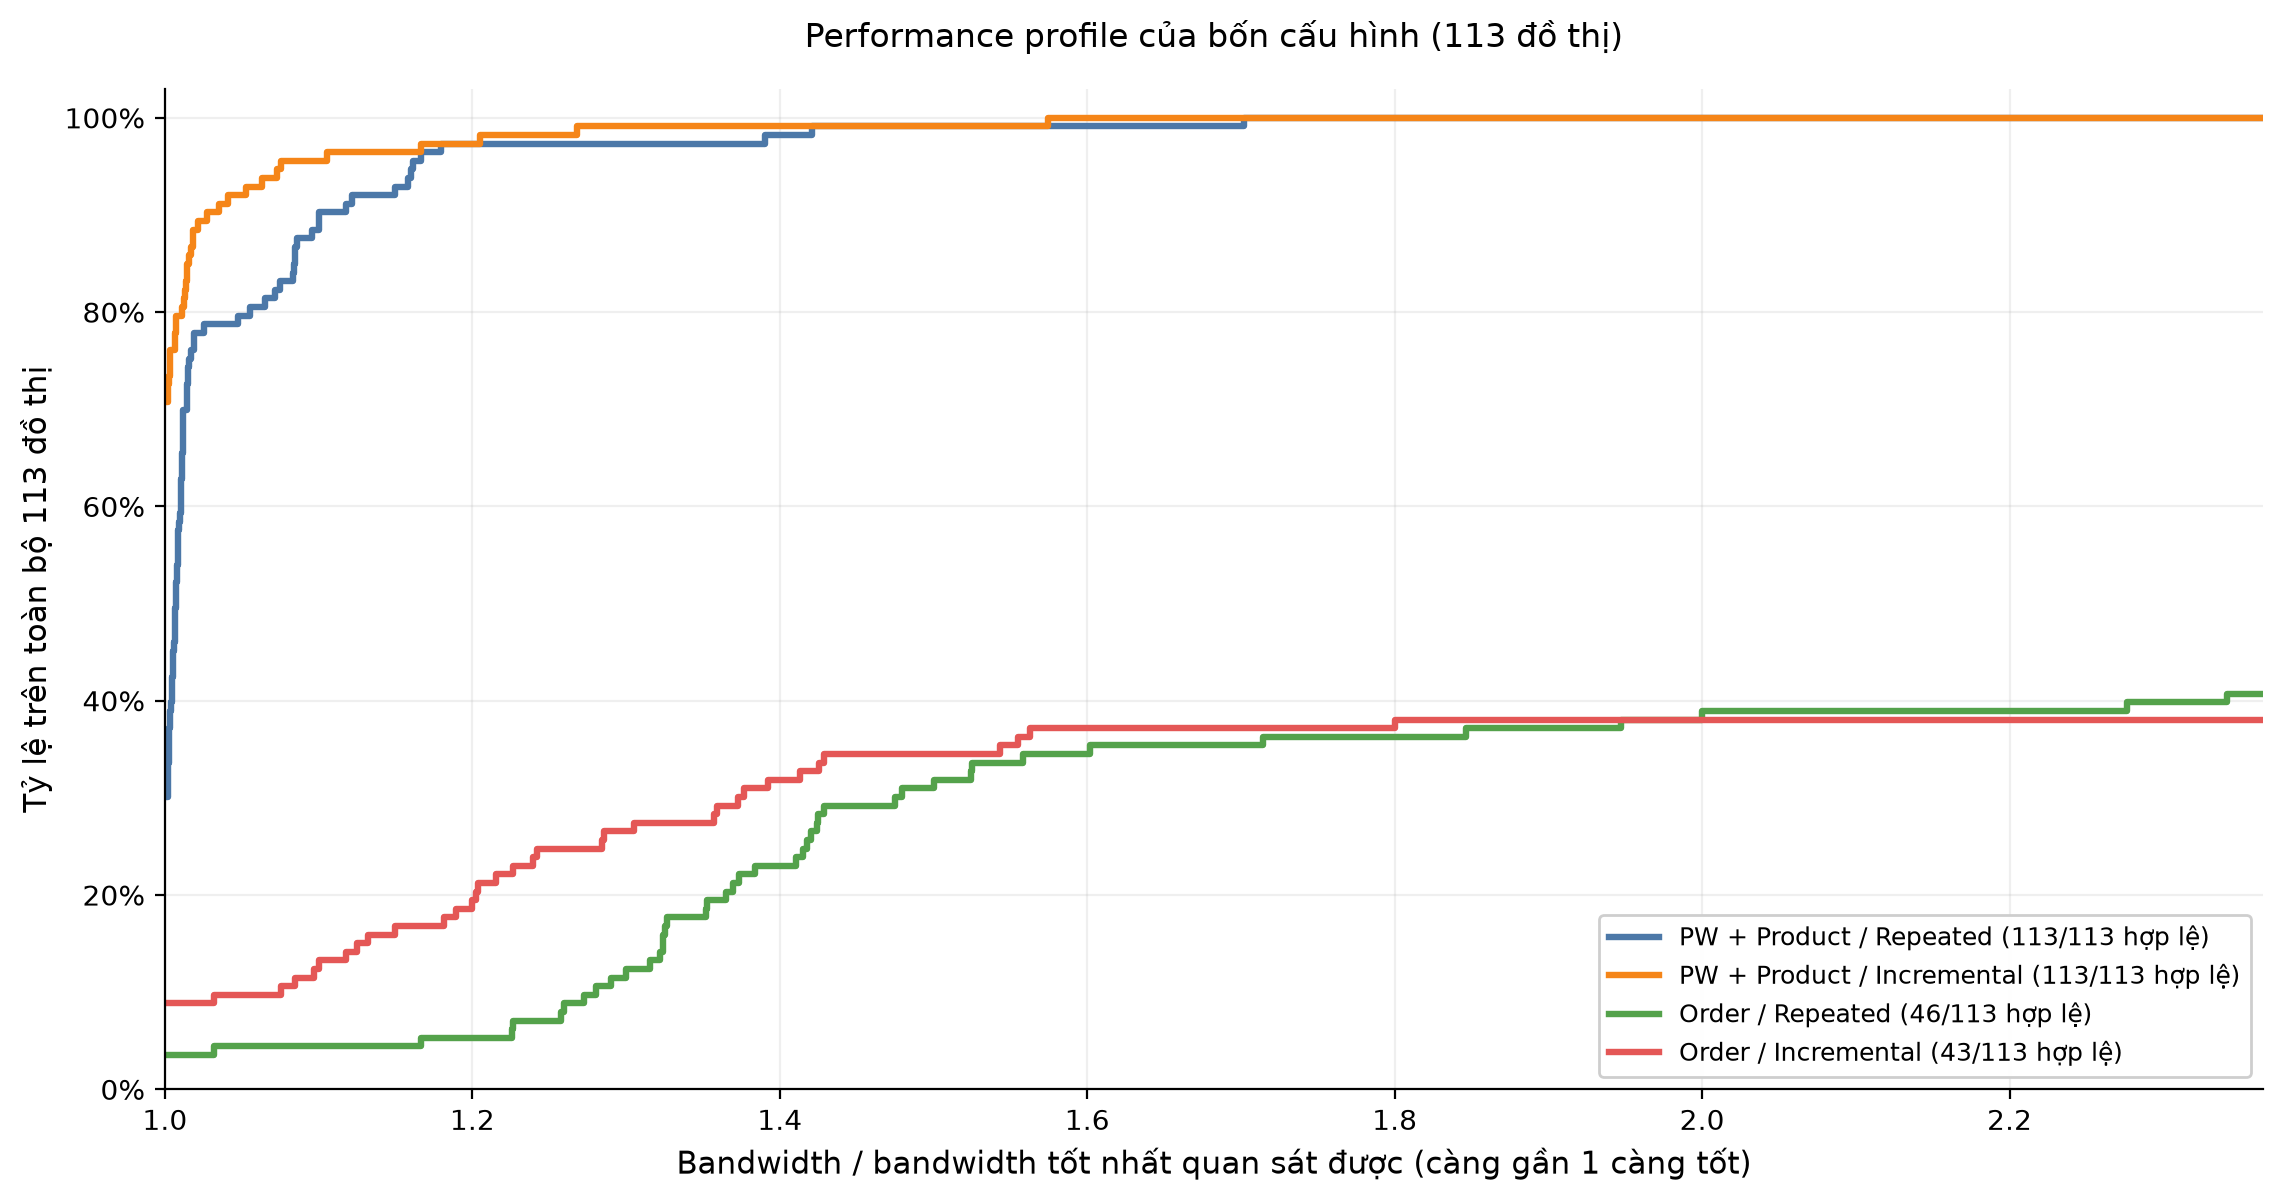
\includegraphics[width=0.90\linewidth]{group1_02_quality_profile.png}
\caption{Performance Profile của bốn cấu hình SAT trên 113 đồ thị. Đường biểu diễn càng cao và càng gần bên trái thể hiện chất lượng nghiệm và mức độ bao phủ càng tốt.}\label{fig:g1-profile}
\end{figure}
\end{minipage}
\par

Theo Hình~\ref{fig:g1-profile}, hai cấu hình Pairwise + Product có chất lượng nghiệm và khả năng bao phủ tốt hơn Order. Đặc biệt, Pairwise + Product + Incremental đạt tỷ lệ cao hơn Repeated ở nhiều mức tỷ số bandwidth. Trong khi đó, hai đường biểu diễn của Order chỉ đạt mức bao phủ thấp do không tìm được nghiệm hợp lệ trên nhiều đồ thị thuộc tập \code{hb_80}.

Để đánh giá trực tiếp ảnh hưởng của chiến lược giải, nhóm tiếp tục so sánh Repeated và Incremental trên cùng những đồ thị mà cả hai đều có nghiệm. Kết quả được trình bày trong Bảng~\ref{tab:g1-pairs}.

\begin{table}[pos=H]
\centering
\caption{So sánh bandwidth giữa Repeated và Incremental trên các đồ thị cùng có nghiệm.}
\label{tab:g1-pairs}
\small
\begin{tabular}{lrrrr}
\toprule
\textbf{Mã hóa} & \textbf{Số đồ thị} & \textbf{Repeated tốt hơn} & \textbf{Hòa} & \textbf{Incremental tốt hơn} \\
\midrule
Pairwise + Product & 113 & 27 & 9 & 77 \\
Order & 43 & 2 & 6 & 35 \\
\bottomrule
\end{tabular}
\end{table}

Với Pairwise + Product, Incremental tìm được bandwidth nhỏ hơn Repeated trên 77 đồ thị, hai phương pháp hòa nhau trên 9 đồ thị và Repeated tốt hơn trên 27 đồ thị. Đối với Order, trong 43 đồ thị mà cả hai chiến lược đều tìm được nghiệm, Incremental tốt hơn trên 35 đồ thị, hòa trên 6 đồ thị và kém hơn trên 2 đồ thị.

\figreport{group1_03_repeated_vs_incremental.png}{0.92}{So sánh bandwidth giữa Repeated và Incremental. Điểm nằm dưới đường chéo cho biết Incremental tìm được bandwidth nhỏ hơn.}{fig:g1-pairs}

Hình~\ref{fig:g1-pairs} minh họa trực tiếp kết quả trên. Trục ngang biểu diễn bandwidth của Repeated, còn trục dọc biểu diễn bandwidth của Incremental. Các điểm nằm dưới đường chéo cho biết Incremental tìm được nghiệm tốt hơn, các điểm nằm trên đường chéo cho biết Repeated tốt hơn và các điểm nằm đúng đường chéo thể hiện hai phương pháp có cùng bandwidth.

Nhìn chung, Incremental cho chất lượng nghiệm tốt hơn trên phần lớn các đồ thị được so sánh. Tuy nhiên, kết quả này không có nghĩa Incremental luôn vượt trội, vì Repeated vẫn tìm được nghiệm tốt hơn trên một số đồ thị.


\subsubsection{Phân tích nguyên nhân Order gặp nhiều lỗi}

Kết quả thực nghiệm cho thấy Order Encoding gặp nhiều lỗi khi xử lý các đồ thị lớn. Nguyên nhân đáng chú ý là số lượng mệnh đề CNF được tạo ra để bảo đảm các đỉnh không chiếm trùng vị trí.

Theo Công thức~\eqref{eq:order-size}, chỉ riêng phần ràng buộc hoán vị của Order đã cần $n\binom{n}{2}$ mệnh đề để ngăn hai đỉnh cùng chiếm một vị trí. Vì số mệnh đề tăng theo bậc ba của số đỉnh $n$, kích thước công thức có thể tăng rất nhanh khi đồ thị lớn.

Chẳng hạn, với đồ thị có 494 đỉnh, phần ràng buộc này đã tạo ra hơn 60 triệu mệnh đề. Khi số đỉnh tăng lên 662, số mệnh đề vượt 144 triệu. Các mệnh đề cần được tạo và lưu trong bộ nhớ trước hoặc trong quá trình nạp vào SAT Solver, khiến lượng RAM sử dụng tăng mạnh.

Trong tổng số 137 lượt ERROR của hai cấu hình Order, có 116 lượt chưa ghi nhận được lần gọi SAT nào, tương ứng với \code{sat\_calls=0}. Điều này cho thấy nhiều lượt chạy bị dừng trước khi bắt đầu giải SAT, trong giai đoạn chuẩn bị mô hình hoặc khởi tạo bộ giải. Kích thước CNF rất lớn cùng các trường hợp vượt RAM đã được ghi nhận cho thấy bộ nhớ là một hạn chế quan trọng của cách cài đặt Order hiện tại.

Như vậy, mặc dù Order Encoding sử dụng $n^2$ biến Boolean và không cần các biến phụ AMO như Pairwise + Product, số lượng mệnh đề của nó vẫn có thể rất lớn. Điều này cho thấy số biến ít hơn không đồng nghĩa với việc công thức SAT sử dụng ít bộ nhớ hơn hoặc giải nhanh hơn.

Để cải thiện hiệu quả của Order, có thể nghiên cứu cách mã hóa ràng buộc hoán vị gọn hơn, giảm số mệnh đề phải tạo và tối ưu việc sử dụng bộ nhớ. Tuy nhiên, đây là những hướng phát triển tiếp theo, chưa được đánh giá trong các thực nghiệm hiện tại.

\subsubsection{Nhận xét và lựa chọn cấu hình SAT}

Từ kết quả thực nghiệm, nhóm lựa chọn Pairwise + Product + Incremental làm cấu hình SAT đại diện để so sánh với các phương pháp CP và MIP. Cấu hình này tìm được nghiệm hợp lệ trên toàn bộ 113 đồ thị và đạt chất lượng bandwidth tốt hơn Repeated trên phần lớn các trường hợp.

Cần lưu ý rằng Incremental có thể tận dụng các mệnh đề và thông tin đã học từ những lần giải trước, nhưng không bảo đảm luôn chạy nhanh hơn Repeated. Hiệu quả thực tế còn phụ thuộc vào kích thước công thức CNF, quá trình xây dựng mệnh đề và cách SAT Solver tìm kiếm nghiệm. Vì vậy, lựa chọn trên dựa vào kết quả chất lượng nghiệm và khả năng giải thành công trong giới hạn tài nguyên của thí nghiệm.

\FloatBarrier


\subsection{So sánh SAT, CP và MIP}

Sau khi lựa chọn Pairwise + Product + Incremental làm cấu hình SAT đại diện, nhóm tiến hành so sánh với bốn phương pháp khác gồm IBM CP Optimizer (CP), IBM CPLEX MIP (MIP), Google OR-Tools CP-SAT và Gurobi. Cả năm phương pháp được thử nghiệm trên 113 đồ thị với giới hạn thời gian 120 giây và bộ nhớ tối đa 8 GiB cho mỗi lượt chạy. Mục tiêu là so sánh khả năng tìm nghiệm, chất lượng bandwidth và khả năng chứng minh tối ưu.

\subsubsection{Kết quả tổng quan}

Bảng~\ref{tab:g3-status} trình bày trạng thái kết quả của năm phương pháp. Trong đó, OPTIMAL là các lượt đã chứng minh được nghiệm tối ưu, FEASIBLE là các lượt tìm được nghiệm hợp lệ nhưng chưa chứng minh tối ưu, TIMEOUT là các lượt chưa tìm được nghiệm trước khi hết thời gian và ERROR là các lượt chạy gặp lỗi.

\begin{table}[pos=H]
\centering
\caption{Kết quả của năm phương pháp trên 113 đồ thị.}
\label{tab:g3-status}
\small
\begin{tabular}{lrrrrr}
\toprule
\textbf{Phương pháp} & \textbf{OPT} & \textbf{FEAS} & \textbf{TO} & \textbf{ERR} & \textbf{Có nghiệm} \\
\midrule
SAT & 5 & 108 & 0 & 0 & 113 \\
CP & 6 & 107 & 0 & 0 & 113 \\
MIP & 1 & 105 & 5 & 2 & 106 \\
CP-SAT & 6 & 106 & 1 & 0 & 112 \\
Gurobi & 1 & 98 & 14 & 0 & 99 \\
\bottomrule
\end{tabular}
\end{table}

Kết quả cho thấy SAT và CP đều tìm được nghiệm hợp lệ trên toàn bộ 113 đồ thị. CP-SAT đạt 112 đồ thị, MIP đạt 106 đồ thị và Gurobi đạt 99 đồ thị. Tổng cộng có 543 lượt tìm được nghiệm hợp lệ, 20 lượt TIMEOUT và 2 lượt ERROR. Hai lượt ERROR của MIP được ghi nhận do vượt giới hạn bộ nhớ 8 GiB.

\figreport{group3_01_status.png}{0.94}{Phân bố trạng thái của năm phương pháp trên toàn bộ 113 đồ thị và hai tập dữ liệu hb\_33, hb\_80.}{fig:g3-status}

Hình~\ref{fig:g3-status} cho thấy phần lớn các trường hợp TIMEOUT và ERROR xuất hiện ở những đồ thị lớn thuộc tập \code{hb_80}. Trong khi đó, SAT và CP vẫn tìm được nghiệm trên toàn bộ dữ liệu. Điều này cho thấy hai phương pháp có khả năng hoàn thành thí nghiệm tốt hơn trong giới hạn tài nguyên đã đặt ra.

\subsubsection{So sánh chất lượng nghiệm}

Để đánh giá chất lượng nghiệm, nhóm so sánh bandwidth mà mỗi phương pháp tìm được với bandwidth nhỏ nhất quan sát được trên cùng một đồ thị. Ngoài ra, nhóm sử dụng khoảng cách tối ưu tương đối (relative gap) để đánh giá mức độ gần nhau giữa cận trên và cận dưới của từng phương pháp.

\begin{table}[pos=H]
\centering
\caption{So sánh chất lượng nghiệm và khoảng cách tối ưu tương đối.}
\label{tab:g3-quality}
\small
\begin{tabular}{lrrr}
\toprule
\textbf{Phương pháp} & \textbf{Có nghiệm} & \textbf{Tốt nhất} & \textbf{Trung vị gap (\%)} \\
\midrule
SAT & 113 & 6 & 86.76 \\
CP & 113 & 113 & 50.98 \\
MIP & 106 & 1 & 90.30 \\
CP-SAT & 112 & 6 & 87.07 \\
Gurobi & 99 & 7 & 81.65 \\
\bottomrule
\end{tabular}
\end{table}

Kết quả cho thấy CP đạt hoặc hòa bandwidth nhỏ nhất quan sát được trên cả 113 đồ thị. Trong khi đó, SAT và CP-SAT cùng đạt mốc này trên 6 đồ thị, Gurobi trên 7 đồ thị và MIP trên 1 đồ thị. Đây là kết quả nổi bật của CP trong thí nghiệm, cho thấy phương pháp này tìm được nghiệm có chất lượng tốt hơn các phương pháp còn lại trên bộ dữ liệu đang xét.

Tuy nhiên, cần phân biệt giữa việc tìm được bandwidth nhỏ nhất quan sát được và việc chứng minh nghiệm tối ưu. Mặc dù CP đạt kết quả tốt nhất trên cả 113 đồ thị, chỉ có 6 lượt được xác nhận OPTIMAL. Những lượt còn lại vẫn có thể tồn tại hoán vị với bandwidth nhỏ hơn nhưng chưa được chứng minh hoặc tìm thấy.

\figreport{group3_02_quality_profile.png}{0.92}{Performance Profile của năm phương pháp trên 113 đồ thị. Tỷ số bandwidth càng gần 1 thì chất lượng nghiệm càng tốt.}{fig:g3-profile}

Hình~\ref{fig:g3-profile} cho thấy đường biểu diễn của CP đạt 100\% ngay tại tỷ số bằng 1, do CP tìm được bandwidth tốt nhất quan sát trên toàn bộ dữ liệu. Các phương pháp còn lại có tỷ số lớn hơn trên nhiều đồ thị, cho thấy bandwidth tìm được thường cao hơn kết quả của CP. Biểu đồ sử dụng thang logarit trên trục ngang để thể hiện rõ sự chênh lệch lớn giữa các phương pháp.

\figreport{group3_03_relative_gap.png}{0.92}{Phân bố khoảng cách tối ưu tương đối của các nghiệm hợp lệ theo từng phương pháp. Gap càng nhỏ thì khoảng cách giữa cận trên và cận dưới càng hẹp.}{fig:g3-gap}

Theo Hình~\ref{fig:g3-gap}, CP có trung vị gap bằng 50,98\%, thấp nhất trong năm phương pháp. Các phương pháp còn lại có trung vị gap từ 81,65\% đến 90,30\%. Kết quả này cho thấy khoảng cách giữa cận trên và cận dưới của CP nhìn chung nhỏ hơn trong thí nghiệm.

Tuy nhiên, gap lớn không nhất thiết có nghĩa nghiệm tìm được quá kém, vì nguyên nhân cũng có thể là cận dưới chưa đủ mạnh. Đồng thời, biểu đồ gap sử dụng tất cả nghiệm hợp lệ của từng phương pháp nên số lượng đồ thị được thống kê có thể khác nhau.

\subsubsection{Một số trường hợp minh họa}

Bảng~\ref{tab:examples} trình bày kết quả trên một số đồ thị tiêu biểu nhằm làm rõ sự khác biệt giữa các phương pháp.

\begin{table}[pos=H]
\centering
\caption{Bandwidth tìm được trên một số đồ thị tiêu biểu.}
\label{tab:examples}
\small
\begin{tabular}{lrrrrrr}
\toprule
\textbf{Đồ thị} & \textbf{$n$} & \textbf{SAT} & \textbf{CP} & \textbf{MIP} & \textbf{CP-SAT} & \textbf{Gurobi} \\
\midrule
pores\_1 & 30 & 7* & 7* & 7* & 7* & 7* \\
bcspwr01 & 39 & 5 & 5 & 6 & 5* & 5 \\
494\_bus & 494 & 424 & 49 & 482 & 195 & TO \\
bcsstk20 & 467 & 413 & 17 & 465 & 170 & 386 \\
nos2 & 638 & 593 & 3* & 609 & 285 & 634 \\
fs\_541\_1 & 541 & 499 & 270* & 521 & 464 & 411 \\
\bottomrule
\end{tabular}
\end{table}

\noindent\footnotesize{Dấu * biểu thị nghiệm được chính lượt chạy đó xác nhận OPTIMAL; TO biểu thị TIMEOUT.}\normalsize

Đáng chú ý, với đồ thị \code{nos2} có 638 đỉnh, CP tìm được và chứng minh bandwidth tối ưu bằng 3, trong khi SAT tìm được 593, MIP là 609, CP-SAT là 285 và Gurobi là 634. Tương tự, trên đồ thị \code{494_bus}, CP tìm được bandwidth 49, nhỏ hơn đáng kể so với các phương pháp còn lại.

Những ví dụ này cho thấy số lượng đỉnh lớn không đồng nghĩa với việc mọi phương pháp đều gặp cùng một mức độ khó. Kết quả còn phụ thuộc vào cấu trúc đồ thị, cách biểu diễn bài toán và chiến lược tìm kiếm của từng bộ giải.

\FloatBarrier


\subsubsection{So sánh mức sử dụng bộ nhớ}

Bên cạnh chất lượng nghiệm, nhóm đánh giá lượng bộ nhớ RAM được sử dụng trong quá trình giải. Chỉ số được lựa chọn là mức RAM cao nhất ghi nhận ở mỗi lượt chạy. Việc thống kê bao gồm cả những lượt TIMEOUT và ERROR, vì các lượt này vẫn tiêu thụ tài nguyên máy tính.

\begin{table}[pos=H]
\centering
\caption{Thống kê mức sử dụng RAM của năm phương pháp trên 113 đồ thị.}
\label{tab:g3-ram}
\small
\begin{tabular}{lrr}
\toprule
\textbf{Phương pháp} & \textbf{RAM trung vị (MiB)} & \textbf{RAM lớn nhất (MiB)} \\
\midrule
SAT & 2241.23 & 4238.11 \\
CP & 147.18 & 452.52 \\
MIP & 1281.11 & 8213.09 \\
CP-SAT & 246.18 & 1805.83 \\
Gurobi & 834.66 & 7653.45 \\
\bottomrule
\end{tabular}
\end{table}

Kết quả cho thấy CP sử dụng ít bộ nhớ nhất, với RAM trung vị khoảng 147 MiB và mức cao nhất khoảng 453 MiB. CP-SAT cũng có mức sử dụng bộ nhớ tương đối thấp, với trung vị khoảng 246 MiB. Trong khi đó, SAT có RAM trung vị khoảng 2241 MiB, cao hơn đáng kể so với hai phương pháp trên.

MIP có mức sử dụng RAM lớn nhất lên tới 8213 MiB, vượt nhẹ giới hạn 8 GiB do khoảng thời gian giữa các lần lấy mẫu bộ nhớ. Gurobi cũng có mức sử dụng RAM khá cao ở một số đồ thị lớn.

\figreport{group3_04_memory.png}{0.94}{So sánh RAM cao nhất được ghi nhận theo phương pháp và kích thước đồ thị. Tam giác rỗng biểu diễn TIMEOUT, dấu X biểu diễn ERROR và đường ngang thể hiện giới hạn 8 GiB.}{fig:g3-ram}

Hình~\ref{fig:g3-ram} cho thấy mức sử dụng RAM thường tăng khi kích thước đồ thị lớn hơn, tuy nhiên tốc độ tăng khác nhau giữa các phương pháp. SAT sử dụng nhiều bộ nhớ để lưu trữ công thức CNF, trong khi các phương pháp MIP có mức RAM thay đổi khá lớn tùy theo đồ thị. Ngược lại, CP duy trì mức sử dụng bộ nhớ tương đối thấp trên bộ dữ liệu thực nghiệm.

\subsubsection{Nhận xét chung}

Từ kết quả thực nghiệm, CP là phương pháp nổi bật nhất khi vừa tìm được nghiệm trên toàn bộ 113 đồ thị, vừa đạt bandwidth nhỏ nhất quan sát được và sử dụng ít bộ nhớ nhất. CP-SAT cũng có khả năng hoàn thành thí nghiệm tốt với mức RAM tương đối thấp.

SAT có ưu điểm là tìm được nghiệm hợp lệ trên toàn bộ dữ liệu, nhưng chất lượng bandwidth còn thấp hơn CP trên phần lớn đồ thị và chi phí bộ nhớ tương đối cao. Các phương pháp MIP và Gurobi vẫn tìm được nghiệm trên nhiều trường hợp, tuy nhiên gặp hạn chế về thời gian hoặc bộ nhớ ở một số đồ thị lớn.

Những kết quả trên phản ánh hiệu quả của các mô hình và bộ giải trong điều kiện thực nghiệm cụ thể. Chúng không có nghĩa một phương pháp luôn tốt hơn các phương pháp khác trên mọi bài toán hoặc mọi cách cấu hình.
\FloatBarrier



\section{Thảo luận và hạn chế}

\subsection{Thảo luận kết quả thực nghiệm}

Kết quả thực nghiệm cho thấy cách mã hóa bài toán có ảnh hưởng lớn đến hiệu quả của SAT Solver. Trong thí nghiệm so sánh năm phương pháp AMO, Product đạt số lần tìm được bandwidth tốt nhất quan sát được cao nhất, trong khi Sequential có nhiều lượt chứng minh tối ưu hơn. Điều này cho thấy không có phương pháp mã hóa nào vượt trội ở mọi tiêu chí. Việc lựa chọn mã hóa cần xem xét đồng thời chất lượng nghiệm, khả năng chứng minh tối ưu và mức sử dụng tài nguyên.

Khi so sánh Pairwise và Order Encoding, Pairwise + Product cho kết quả ổn định hơn trên các đồ thị lớn. Trong khi đó, Order gặp nhiều lỗi do số lượng mệnh đề CNF tăng nhanh theo số đỉnh, dẫn đến nhu cầu bộ nhớ lớn. Kết quả này cho thấy số biến Boolean ít hơn không đồng nghĩa với việc một cách mã hóa sử dụng ít RAM hoặc giải nhanh hơn.

Đối với hai chiến lược SAT, Incremental có ưu điểm là tái sử dụng solver và các mệnh đề đã học từ những lần giải trước. Trong phiên bản cải tiến, chương trình chỉ xây dựng CNF đầy đủ ở ngưỡng ban đầu, sau đó trực tiếp sinh các mệnh đề cạnh cần bổ sung khi giảm ngưỡng bandwidth. Cách triển khai này giúp giảm chi phí xây dựng CNF. Tuy nhiên, việc giảm thời gian xây dựng không bảo đảm chất lượng nghiệm hoặc thời gian giải luôn tốt hơn, vì quá trình tìm kiếm còn phụ thuộc vào cách solver xử lý các mệnh đề.

Trong thí nghiệm so sánh các bộ giải, IBM CP Optimizer đạt kết quả nổi bật nhất khi tìm được bandwidth nhỏ nhất quan sát được trên toàn bộ 113 đồ thị và sử dụng ít bộ nhớ nhất. SAT cũng tìm được nghiệm hợp lệ trên toàn bộ dữ liệu, nhưng chất lượng bandwidth nhìn chung thấp hơn CP. Kết quả cho thấy cách biểu diễn bài toán và cơ chế tìm kiếm của từng bộ giải có ảnh hưởng đáng kể đến hiệu quả giải.

\subsection{Hạn chế của thực nghiệm}

Mặc dù đã so sánh nhiều phương pháp, thực nghiệm vẫn có một số hạn chế. Trước hết, mỗi cấu hình chỉ được chạy một lần trên từng đồ thị, chưa thực hiện nhiều lần với các thiết lập ngẫu nhiên khác nhau. Vì vậy, kết quả chủ yếu phản ánh hiệu quả quan sát được trong điều kiện thử nghiệm, chưa đủ cơ sở để đánh giá độ ổn định giữa nhiều lần chạy.

Bên cạnh đó, mỗi lượt chạy được giới hạn 120 giây và 8 GiB bộ nhớ. Một số phương pháp có thể tiếp tục cải thiện nghiệm hoặc chứng minh tối ưu nếu được cấp thêm tài nguyên. Do đó, các kết quả FEASIBLE chưa chắc là nghiệm tốt nhất mà phương pháp có thể tìm được nếu không bị giới hạn thời gian.

Ngoài ra, các biểu đồ đánh giá chất lượng nghiệm được xây dựng từ những kết quả hợp lệ đã ghi nhận. Các lượt TIMEOUT và ERROR có thể làm giảm số lượng đồ thị được sử dụng trong một số phép so sánh. Vì vậy, cần xem xét đồng thời chất lượng nghiệm và khả năng hoàn thành thí nghiệm để tránh đánh giá thiếu chính xác.

\section{Kết luận}

Trong báo cáo này, nhóm đã nghiên cứu và triển khai phương pháp giải bài toán Bandwidth Minimization Problem (BMP) bằng SAT, tập trung vào hai cách mã hóa Pairwise và Order, năm kỹ thuật mã hóa AMO cùng hai chiến lược Repeated SAT và Incremental SAT. Đồng thời, nhóm sử dụng các bộ giải CP, CP-SAT, CPLEX MIP và Gurobi để đối chiếu hiệu quả trên cùng bộ dữ liệu gồm 113 đồ thị.

Kết quả thực nghiệm cho thấy Product là phương pháp mã hóa AMO phù hợp với mục tiêu tìm nghiệm bandwidth tốt trong điều kiện khảo sát, còn Sequential có số lượt chứng minh tối ưu cao hơn. Trong các cấu hình SAT, Pairwise + Product hoạt động ổn định hơn Order, đặc biệt trên những đồ thị lớn. Chiến lược Incremental cũng cho thấy lợi ích trong việc tái sử dụng thông tin giải, mặc dù hiệu quả còn phụ thuộc vào cách triển khai và đặc điểm từng đồ thị.

Khi so sánh với các phương pháp đối chứng, IBM CP Optimizer đạt hoặc hòa bandwidth nhỏ nhất quan sát được trên cả 113 đồ thị, đồng thời có mức sử dụng RAM thấp nhất. SAT vẫn tìm được nghiệm hợp lệ trên toàn bộ dữ liệu nhưng còn hạn chế về chất lượng nghiệm và chi phí xây dựng công thức CNF đối với các trường hợp lớn.

Nhìn chung, kết quả cho thấy việc lựa chọn cách mã hóa và chiến lược giải có ảnh hưởng lớn đến hiệu quả giải BMP. Các thực nghiệm đã làm rõ ưu điểm, hạn chế của từng phương pháp và cung cấp cơ sở để đánh giá khả năng ứng dụng SAT trong bài toán tối ưu bandwidth.

\section*{Công khai dữ liệu và mã nguồn (Data Availability)}
Kho mã được cấu hình trong dự án là
\begin{center}\url{https://github.com/NhHung07/Bandwidth-Minimization-Problem}\end{center}

\section*{Tuyên bố về việc sử dụng AI sinh trong viết báo cáo}
Trong quá trình chuẩn bị bản thảo này, tác giả đã sử dụng các mô hình ngôn ngữ lớn (OpenAI ChatGPT và Google Gemini) nhằm hỗ trợ rà soát ngữ pháp, cấu trúc hóa văn bản và định dạng mã nguồn LaTeX. Sau quá trình sinh bản thảo ban đầu, tác giả đã trực tiếp kiểm tra, xác thực toàn bộ các công thức toán học, mã nguồn thuật toán, dữ liệu bảng biểu thực nghiệm và hình vẽ, đồng thời chịu toàn bộ trách nhiệm về tính trung thực và độ chính xác của bài báo cáo.

\begin{thebibliography}{99}
\bibitem{hungNQueens}
Phạm Đức Hùng, \emph{Nghiên cứu Giải Bài toán NQueens bằng SAT: Đánh giá Thực nghiệm 5 Kỹ thuật Mã hóa CNF và So sánh Đa Mô hình với ILP và CP}, báo cáo giữa kỳ do tác giả cung cấp, tệp \code{NQueens.pdf}, 12 trang.
\bibitem{torres2015}
J. Torres-Jimenez, I. Izquierdo-Marquez, A. Garcia-Robledo, A. Gonzalez-Gomez, J. Bernal, R. N. Kacker,
A dual representation simulated annealing algorithm for the bandwidth minimization problem on graphs,
\emph{Information Sciences} 303 (2015) 33--49. \url{https://doi.org/10.1016/j.ins.2014.12.041}.
\bibitem{pysat}
A. Ignatiev, A. Morgado, J. Marques-Silva, PySAT: A Python toolkit for prototyping with SAT oracles,
\emph{SAT 2018}, 428--437. \url{https://doi.org/10.1007/978-3-319-94144-8_26}.
\bibitem{sinz}
C. Sinz, Towards an optimal CNF encoding of Boolean cardinality constraints,
\emph{CP 2005}, 827--831. \url{https://doi.org/10.1007/11564751_73}.
\bibitem{commander}
W. Klieber, G. Kwon, Efficient CNF encoding for selecting 1 from N objects,
\emph{Workshop on Constraints in Formal Verification}, 2007.
\url{https://www.cs.cmu.edu/~wklieber/papers/2007_efficient-cnf-encoding-for-selecting-1.pdf}.
\bibitem{product}
SAT4J, \emph{Product encoding API}, mô tả mã hóa 2-product của J. Chen và tham chiếu bài gốc năm 2010.
\url{https://www.sat4j.org/maven23/org.sat4j.core/apidocs/org/sat4j/tools/encoding/Product.html}. Truy cập ngày 18/11/2026.
\bibitem{ortools}
Google, \emph{OR-Tools: CP-SAT Solver}, tài liệu chính thức.
\url{https://developers.google.com/optimization/cp/cp_solver}. Truy cập ngày 18/11/2026.
\bibitem{ibmcp}
IBM, \emph{IBM ILOG CPLEX Optimization Studio: CP Optimizer}, tài liệu chính thức.
\url{https://www.ibm.com/docs/en/icos/22.1.1}. Truy cập ngày 18/11/2026.
\bibitem{ibmmip}
IBM, \emph{Emphasizing feasibility and optimality}, tài liệu tham số MIP.
\url{https://www.ibm.com/docs/en/icos/22.1.1?topic=optimizer-emphasizing-feasibility-optimality}. Truy cập ngày 18/11/2026.
\bibitem{gurobi}
Gurobi Optimization, \emph{Parameter Guidelines}, tài liệu chính thức.
\url{https://docs.gurobi.com/projects/optimizer/en/current/concepts/parameters/guidelines.html}. Truy cập ngày 18/11/2026.
\end{thebibliography}
\end{document}
